\setcounter{section}{34}
\section{Мосты, точки сочленения. Введение функции ret. Критерий того, что ребро является мостом.}
Пусть G - связный граф\\
\textbf{Определение} Ребро $e \in E(G)$ называется \textit{мостом}, если G-e (граф без ребра е) - несвязен
\\
\\
\textbf{Определение} Вершина v называется \textit{точкой сочленения}, если G-v - несвязен
\\
\\
Введем функцию ret[v] = min(tin[v], tin[u]). Что такое u? Пусть дана вершина v, из которой мы спускаемся по древесным ребрам в вершину w. Тогда какая-то вершинка, в которую мы прыгнем по обратному ребру - вершина u
\begin{center}
    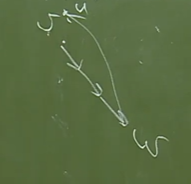
\includegraphics[width=3cm]{images/35-36_alg19.PNG}
\end{center}
Для чего нам это надо. Рассмотрим ret[v]. Что значит, что ребро (u,v) - мост? Значит, мы не можем прыгнуть из области, куда мы спустились по этому ребру, куда-то выше. То есть ret[v] = tin[v]
\\
\begin{center}
    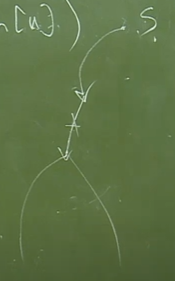
\includegraphics[width=3cm]{images/35-36_algo20.PNG}    
\end{center}

Заметим, что если ребро не древесное, то оно точно не является мостом, так как мы просто удалили какое-то ребро из вершины в предка
\begin{center}
    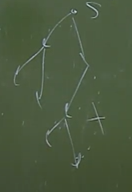
\includegraphics[width=3cm]{images/35-36_alg21.PNG}    
\end{center}

\textbf{Критерий}
e - мост $\Longleftrightarrow$ ret[v] $\geq$ tin[v]
\\
$\blacktriangle \\ \rightarrow \ $ Если ret[v] < tin[v], то нашлась вершинка, в которую можно вернуться по обратным ребрам, если мы спустились ниже ребра (u,v) в дереве dfs, а значит, если убрать это ребро, найдется путь в вершинки ниже этого ребра из вершинок выше этого ребра, то есть связность не нарушится, тогда (u,v) - не мост\\ \\
 $\leftarrow \ $ Если ret[v] $\geq$ tin[v], то из вершин ниже ребра  (u,v) нельзя вернуться в вершины, выше (u,v), а значит, удалив ребро (u,v), мы потеряем связность. Таким образом, (u,v) - мост $\ \blacksquare$
\setcounter{section}{35}
\section{Насчёт ret в неориентированном графе, нахождение мостов}
\begin{verbatim}
void dfs(int v, int p=-1){
    tin[v] =timer++;
    ret[v] = tin[v];
    used[v] = true;
    for(int to: g[v]){
        if(to == p) continue;
        if(used[to]){
            ret[v] = min(ret[v], tin[to]);
        }else{
            dfs(to,v);
             ret[v] = min(ret[v], ret[to]);
             if(ret[to] >=tin[to]) (v, to) - мост
            
        }
    }

}
\end{verbatim}